\section{mo\-Easy\-Cool\-Sched Class Reference}
\label{classmo_easy_cool_sched}\index{moEasyCoolSched@{moEasyCoolSched}}
One of the possible {\bf mo\-Cool\-Sched}{\rm (p.\,\pageref{classmo_cool_sched})}.  


{\tt \#include $<$mo\-Easy\-Cool\-Sched.h$>$}

Inheritance diagram for mo\-Easy\-Cool\-Sched::\begin{figure}[H]
\begin{center}
\leavevmode
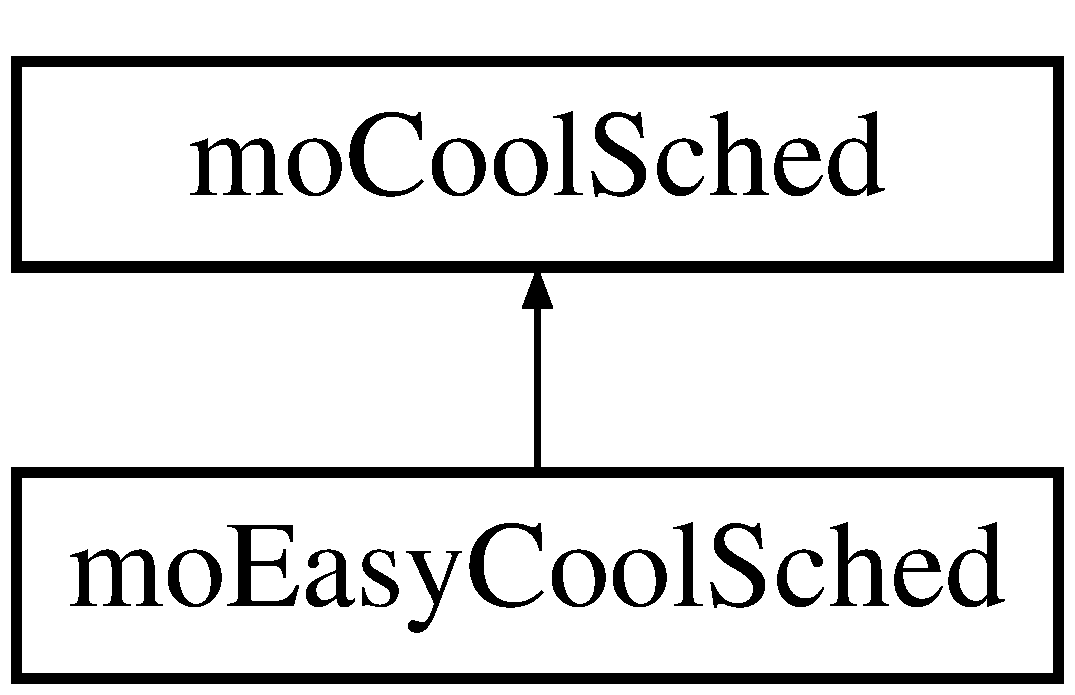
\includegraphics[height=2cm]{classmo_easy_cool_sched}
\end{center}
\end{figure}
\subsection*{Public Member Functions}
\begin{CompactItemize}
\item 
{\bf mo\-Easy\-Cool\-Sched} (double \_\-\_\-threshold, double \_\-\_\-ratio)
\begin{CompactList}\small\item\em Simple constructor. \item\end{CompactList}\item 
bool {\bf operator()} (double \&\_\-\_\-temp)
\begin{CompactList}\small\item\em Function which proceeds to the cooling. \item\end{CompactList}\end{CompactItemize}
\subsection*{Private Attributes}
\begin{CompactItemize}
\item 
double {\bf threshold}\label{classmo_easy_cool_sched_3dd53700390b7bb6428db80e01626c83}

\begin{CompactList}\small\item\em The temperature threhold. \item\end{CompactList}\item 
double {\bf ratio}\label{classmo_easy_cool_sched_1f84deff87defafd927e8c323b188f38}

\begin{CompactList}\small\item\em The decreasing factor of the temperature. \item\end{CompactList}\end{CompactItemize}


\subsection{Detailed Description}
One of the possible {\bf mo\-Cool\-Sched}{\rm (p.\,\pageref{classmo_cool_sched})}. 

The simpliest, the temperature decrease according to a ratio until it greater than a threshold. 



Definition at line 22 of file mo\-Easy\-Cool\-Sched.h.

\subsection{Constructor \& Destructor Documentation}
\index{moEasyCoolSched@{mo\-Easy\-Cool\-Sched}!moEasyCoolSched@{moEasyCoolSched}}
\index{moEasyCoolSched@{moEasyCoolSched}!moEasyCoolSched@{mo\-Easy\-Cool\-Sched}}
\subsubsection{\setlength{\rightskip}{0pt plus 5cm}mo\-Easy\-Cool\-Sched::mo\-Easy\-Cool\-Sched (double {\em \_\-\_\-threshold}, double {\em \_\-\_\-ratio})\hspace{0.3cm}{\tt  [inline]}}\label{classmo_easy_cool_sched_c556b41343700293bb17e3b20d81e0f2}


Simple constructor. 

\begin{Desc}
\item[Parameters:]
\begin{description}
\item[{\em \_\-\_\-threshold}]the threshold. \item[{\em \_\-\_\-ratio}]the ratio used to descrease the temperature. \end{description}
\end{Desc}


Definition at line 31 of file mo\-Easy\-Cool\-Sched.h.

\subsection{Member Function Documentation}
\index{moEasyCoolSched@{mo\-Easy\-Cool\-Sched}!operator()@{operator()}}
\index{operator()@{operator()}!moEasyCoolSched@{mo\-Easy\-Cool\-Sched}}
\subsubsection{\setlength{\rightskip}{0pt plus 5cm}bool mo\-Easy\-Cool\-Sched::operator() (double \& {\em \_\-\_\-temp})\hspace{0.3cm}{\tt  [inline]}}\label{classmo_easy_cool_sched_ca08df878417ef1124e6933a9c2d7a0b}


Function which proceeds to the cooling. 

Decrease the temperature and indicates if it is greater than the threshold.

\begin{Desc}
\item[Parameters:]
\begin{description}
\item[{\em \_\-\_\-temp}]the current temperature. \end{description}
\end{Desc}
\begin{Desc}
\item[Returns:]if the new temperature (current temperature $\ast$ ratio) is greater than the threshold. \end{Desc}


Definition at line 44 of file mo\-Easy\-Cool\-Sched.h.

References ratio, and threshold.

The documentation for this class was generated from the following file:\begin{CompactItemize}
\item 
mo\-Easy\-Cool\-Sched.h\end{CompactItemize}
